\documentclass[aspectratio=169]{beamer}

\usetheme[progressbar=frametitle]{metropolis}
\usepackage{appendixnumberbeamer}
\usepackage{booktabs}
\usepackage[scale=2]{ccicons}
\usepackage{xspace}
\usepackage{caption}
\usepackage{subcaption}
\usepackage{amsmath, amssymb}

\title{Лекция 3. Линейная регрессия}
\date{Введение в нейронные сети | 17.10.2023}

\begin{document}

\maketitle

\begin{frame}{Линейные модели}
    \begin{itemize}
        \item \textbf{Линейная регрессия}
        \item Линейные классификаторы
    \end{itemize}

    Сегодня будем разбираться с линейной регрессией.
\end{frame}

\begin{frame}{Как формализовывать задачу?}
    
\includegraphics[width=\linewidth]{figures/fig1.jpg}
\end{frame}

\begin{frame}{Формализация задачи}
    \begin{itemize}
        \item \textbf{Постановка задачи}
        \item Данные
        \item Модель (семейство алгоритмов)
        \item Оценка качества (функционал ошибки)
        \item Метод обучения
    \end{itemize}
\end{frame}

\begin{frame}{Постановка задачи}
    Перенесемся в начало XIX века.
    \vfill
    \begin{columns}
        \begin{column}{.4\linewidth}
            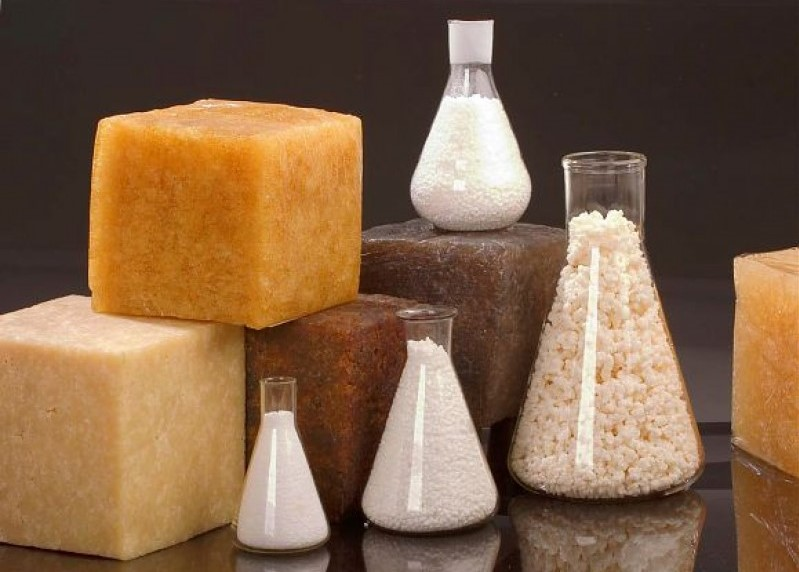
\includegraphics[width=\linewidth]{figures/fig2.jpg}
        \end{column}
        \begin{column}{.6\linewidth}
            \small
            \begin{itemize}
                \item Вы инженер-физик, у вас на столе лежит кусок неизвестного гибкого материала,
                который вы хотите использовать в своем устройстве
                \item Однако, вы не знаете его коэффициента растяжения, и не можете рассчитать
                возникающие силы
                \item Вы хотите построить зависимость силы упругости от растяжения для этого
                материала (и узнать коэффициент растяжения)
            \end{itemize}
        \end{column}
    \end{columns}
\end{frame}

\begin{frame}{Формализация задачи}
    \begin{itemize}
        \item \textbf{Постановка задачи: регрессия, предсказать \( F \) по \( x \)}
        \item Данные
        \item Модель (семейство алгоритмов)
        \item Оценка качества (функционал ошибки)
        \item Метод обучения
    \end{itemize}
\end{frame}

\begin{frame}{Формализация задачи}
    \begin{itemize}
        \item Постановка задачи: регрессия, предсказать \( F \) по \( x \)
        \item \textbf{Данные}
        \item Модель (семейство алгоритмов)
        \item Оценка качества (функционал ошибки)
        \item Метод обучения
    \end{itemize}
\end{frame}

\begin{frame}{Данные}
    Вы проводите некоторое количество измерений и заносите все в табличку подобного вида:
    \begin{center}
        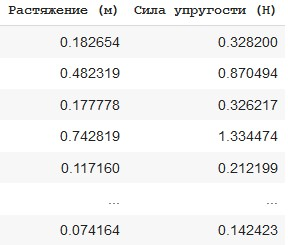
\includegraphics[width=.42\linewidth]{figures/fig3.jpg}
    \end{center}
\end{frame}

\begin{frame}{Формализация задачи}
    \begin{itemize}
        \item Постановка задачи: регрессия, предсказать \( F \) по \( x \)
        \item \textbf{Данные: одномерные (единственный признак \( x \))}
        \item Модель (семейство алгоритмов)
        \item Оценка качества (функционал ошибки)
        \item Метод обучения
    \end{itemize}
\end{frame}

\begin{frame}{Формализация задачи}
    \begin{itemize}
        \item Постановка задачи: регрессия, предсказать \( F \) по \( x \)
        \item Данные: одномерные (единственный признак \( x \))
        \item \textbf{Модель (семейство алгоритмов)}
        \item Оценка качества (функционал ошибки)
        \item Метод обучения
    \end{itemize}
\end{frame}

\begin{frame}{Модель}
    Благодаря Роберту Гуку вы знаете, что сила упругости зависит от растяжения линейно:
    {\LARGE \[ F = k x \]}
    \pause
    Общий вид линейной функции одной переменной:
    {\LARGE \[ y(x) = w_1 x + w_0 \]}
    \pause
    Таким образом, ваша задача среди всех таких функций (семейства) найти ту конкретную,
    которая лучше всего вам подходит (определить параметры)
\end{frame}

\begin{frame}{Формализация задачи}
    \begin{itemize}
        \item Постановка задачи: регрессия, предсказать \( F \) по \( x \)
        \item Данные: одномерные (единственный признак \( x \))
        \item \textbf{Модель: линейная функция одного аргумента}
        \item Оценка качества (функционал ошибки)
        \item Метод обучения
    \end{itemize}
\end{frame}

\begin{frame}{Формализация задачи}
    \centering
    {\Large Что значит ``лучше всего вам подходит''?}
\end{frame}

\begin{frame}{Формализация задачи}
    \centering
    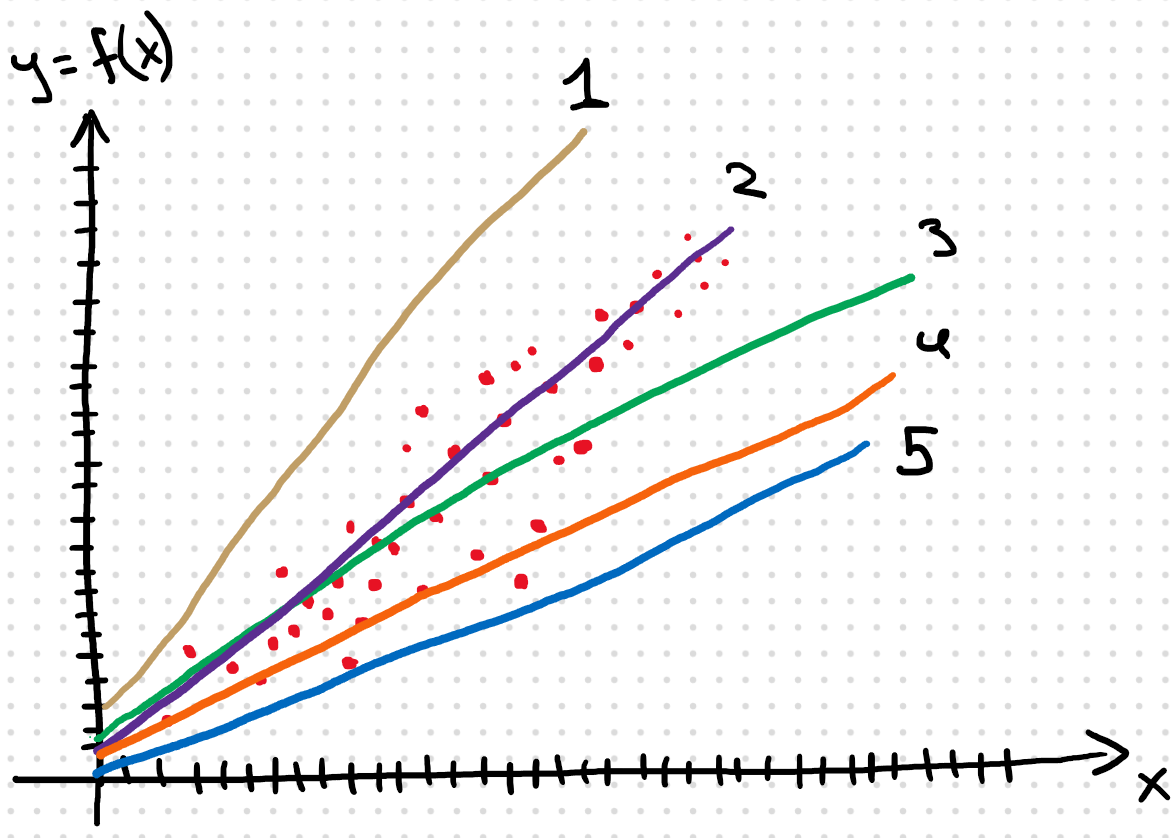
\includegraphics[width=.54\linewidth]{figures/fig4.png} \\
    Какая из функций лучше?
\end{frame}

\begin{frame}{Формализация задачи}
    \begin{itemize}
        \item Постановка задачи: регрессия, предсказать \( F \) по \( x \)
        \item Данные: одномерные (единственный признак \( x \))
        \item Модель: линейная функция одного аргумента
        \item \textbf{Оценка качества (функционал ошибки)}
        \item Метод обучения
    \end{itemize}
\end{frame}

\begin{frame}{Функционалы ошибок}
    Функционал ошибки --- функция \( \mathcal{L}(y, \hat{y}) \), значение
    которой показывает, насколько хороши предсказания модели относительно
    правильных ответов.
    \pause

    Наиболее популярные для задачи регрессии:
    {\large
        \[ MSE(y, \hat{y}) = \frac{1}{n} \sum_{i=1}^n {(y_i - \hat{y_i})}^2 \]
        \[ MAE (y, \hat{y}) = \frac{1}{n} \sum_{i=1}^n {|y_i - \hat{y_i}|} \]
    }
    Ещё есть MSLE, MAPE, SMAPE, и т.д.

    Мы в ближайшее время будем использовать MSE, поскольку она имеет хорошие
    математические свойства.
\end{frame}

\begin{frame}{Формализация задачи}
    \begin{itemize}
        \item Постановка задачи: регрессия, предсказать \( F \) по \( x \)
        \item Данные: одномерные (единственный признак \( x \))
        \item Модель: линейная функция одного аргумента
        \item \textbf{Функционал ошибки: MSE}
        \item Метод обучения
    \end{itemize}
\end{frame}

\begin{frame}{Формализация задачи}
    \begin{itemize}
        \item Постановка задачи: регрессия, предсказать \( F \) по \( x \)
        \item Данные: одномерные (единственный признак \( x \))
        \item Модель: линейная функция одного аргумента
        \item Функционал ошибки: MSE
        \item \textbf{Метод обучения}
    \end{itemize}
\end{frame}

\begin{frame}{Метод обучения}
    Обучение линейной регрессии: подбор таких параметров \( w_0, w_1 \), чтобы результирующая
    функция давала наименьшее значение MSE, то есть
    {\Large
        \[ \frac{1}{n} \sum_{i=1}^n {(y_i - \hat{y_i})}^2 \rightarrow \min_{w_0, w_1} \]
        \pause
        \[ \frac{1}{n} \sum_{i=1}^n {(y_i - w_1 x_i - w_0 )}^2 \rightarrow \min_{w_0, w_1} \]
    }
    Как это сделать?
\end{frame}

\begin{frame}{Метод обучения: (не)много матана}
    Матанализ: в точке экстремума функции производная обращается в ноль
    {\LARGE \[
        \begin{cases}
            \frac{d}{dw_0} \frac{1}{n} \sum_{i=1}^n {(y_i - w_1 x_i - w_0)}^2 = 0 \\
            \frac{d}{dw_1} \frac{1}{n} \sum_{i=1}^n {(y_i - w_1 x_i - w_0)}^2 = 0 
        \end{cases}
    \]}
\end{frame}

\begin{frame}{Метод обучения: (не)много матана}
    \large
    \[
        \frac{d}{dw_0} \frac{1}{n} \sum_{i=1}^n {(y_i - w_1 x_i - w_0)}^2 =
        \frac{d}{dw_0} \sum_{i=1}^n {(y_i - w_1 x_i - w_0)}^2 =
    \]
    \pause
    \[
        = \sum_{i=1}^n \frac{d}{dw_0} {(y_i - w_1 x_i - w_0)}^2 =
        \sum_{i=1}^n 2 {(y_i - w_1 x_i - w_0)(-1)} = 0
    \]
    \pause
    \[
        \Rightarrow \sum_{i=1}^n (y_i - w_1 x_i - w_0) =
        \sum_{i=1}^n y_i - w_1 \sum_{i=1}^n x_i - n w_0 = 0
    \]
    \pause
    \[
        \Rightarrow n w_0 = \sum_{i=1}^n y_i - w_1 \sum_{i=1}^n x_i
    \]
\end{frame}

\begin{frame}{Метод обучения: (не)много матана}
    \large
    \[ \frac{d}{dw_1} \frac{1}{n} \sum_{i=1}^n {(y_i - w_1 x_i - w_0)}^2 = \]
    \pause
    \[
        = \sum_{i=1}^n \frac{d}{dw_1} {(y_i - w_1 x_i - w_0)}^2 =
        \sum_{i=1}^n 2 {(y_i - w_1 x_i - w_0)(-x_i)} = 0
    \]
    \pause
    \[
        \Rightarrow \sum_{i=1}^n x_i {(y_i - w_1 x_i - w_0)} = 0 
    \]
    \pause
    \[
        \Rightarrow w_1 \sum_{i=1}^n x_i^2 = \sum_{i=1}^n x_i y_i -
        w_0 \sum_{i=1}^n x_i   
    \]
\end{frame}

\begin{frame}{Метод обучения: немного матана}
    \LARGE
    \[
        \begin{cases}
            n w_0 = \sum_{i=1}^n y_i - w_1 \sum_{i=1}^n x_i \\
            w_1 \sum_{i=1}^n x_i^2 = \sum_{i=1}^n x_i y_i -
            w_0 \sum_{i=1}^n x_i
        \end{cases}
    \]

    {\large Запишите эту систему, она нам еще понадобится на семинаре}
\end{frame}

\begin{frame}{Формализация задачи}
    \begin{itemize}
        \item Постановка задачи: регрессия, предсказать \( F \) по \( x \)
        \item Данные: одномерные (единственный признак \( x \))
        \item Модель: линейная функция одного аргумента
        \item Функционал ошибки: MSE
        \item \textbf{Метод обучения: аналитическое решение системы уравнений}
    \end{itemize}
\end{frame}

\begin{frame}{Формализация задачи}
    \begin{itemize}
        \item Постановка задачи: регрессия, предсказать \( F \) по \( x \)
        \item Данные: одномерные (единственный признак \( x \))
        \item Модель: линейная функция одного аргумента
        \item Функционал ошибки: MSE
        \item Метод обучения: аналитическое решение системы уравнений
    \end{itemize}

    Численно рассчитаем этот пример на семинаре, а сейчас разберем многомерную регрессию
\end{frame}

\begin{frame}{Многомерная регрессия}
    Рассмотрим случай многомерной (множественной) регрессии --- когда функция зависит больше чем
    от одного входного признака.

    Каждый пример \( x \) теперь вектор в d-мерном пространстве
    \[ \vec{x} = {(x_1, x_2, \ldots, x_d)} \]

    Как будет выглядеть линейная модель в данном случае?
    \[ f(\vec{x}) = f(x_1, x_2, \ldots) = \]
    \pause
    \[ = w_0 + w_1 x_1 + w_2 x_2 + \cdots + w_d x_d = w_0 + \sum_{j=1}^d w_j x_j \]
\end{frame}

\begin{frame}{Bias trick}
    \LARGE
    \[ w_0 + \sum_{j=1}^d w_j x_j = \pause{} w_0 + \langle \vec{w}, \vec{x} \rangle = \]
    \pause
    \[ = \langle \vec{w}, \vec{x} \rangle + w_0 \cdot 1 = \langle \vec{w'}, \vec{x'} \rangle \]
    \[ \vec{x'} = (1, x_1, x_2, \dots, x_d) \quad \vec{w'} = (w_0, w_1, \dots, w_d) \]
\end{frame}

\begin{frame}{Многомерная регрессия}
    Для всей выборки получаем
    {\Large
        \[ \vec{y} = X \vec{w} \]
        \[ \vec{y} = (y_1, y_2, \dots, y_N) \quad \vec{w} = (w_0, w_1, \dots, w_d) \]
        \[
            X = \begin{bmatrix}
                1 & x_{11} & \cdots & x_{1d} \\
                \vdots & \vdots & \ddots & \vdots \\
                1 & x_{N1} & \cdots & x_{Nd}
            \end{bmatrix}
        \]
    }
\end{frame}

\begin{frame}{Аналитическое решение}
    \LARGE
    \[ \frac{1}{N} \| X \vec{w} - \vec{y} \|^2 \rightarrow \min_{\vec{w}} \]
    \pause
    \[ \frac{d}{d \vec{w}} \| X \vec{w} - \vec{y} \|^2 = 0 \]
    \pause
    \[
        \vec{w}^* = \underset{\vec{w}}{\arg\min} \| X \vec{w} - \vec{y} \|^2
        = {(X^T X)}^{-1} X^T \vec{y}
    \]
\end{frame}

\end{document}